% Options for packages loaded elsewhere
\PassOptionsToPackage{unicode}{hyperref}
\PassOptionsToPackage{hyphens}{url}
\PassOptionsToPackage{dvipsnames,svgnames,x11names}{xcolor}
%
\documentclass[
  letterpaper,
  DIV=11,
  numbers=noendperiod]{scrartcl}

\usepackage{amsmath,amssymb}
\usepackage{iftex}
\ifPDFTeX
  \usepackage[T1]{fontenc}
  \usepackage[utf8]{inputenc}
  \usepackage{textcomp} % provide euro and other symbols
\else % if luatex or xetex
  \usepackage{unicode-math}
  \defaultfontfeatures{Scale=MatchLowercase}
  \defaultfontfeatures[\rmfamily]{Ligatures=TeX,Scale=1}
\fi
\usepackage{lmodern}
\ifPDFTeX\else  
    % xetex/luatex font selection
\fi
% Use upquote if available, for straight quotes in verbatim environments
\IfFileExists{upquote.sty}{\usepackage{upquote}}{}
\IfFileExists{microtype.sty}{% use microtype if available
  \usepackage[]{microtype}
  \UseMicrotypeSet[protrusion]{basicmath} % disable protrusion for tt fonts
}{}
\makeatletter
\@ifundefined{KOMAClassName}{% if non-KOMA class
  \IfFileExists{parskip.sty}{%
    \usepackage{parskip}
  }{% else
    \setlength{\parindent}{0pt}
    \setlength{\parskip}{6pt plus 2pt minus 1pt}}
}{% if KOMA class
  \KOMAoptions{parskip=half}}
\makeatother
\usepackage{xcolor}
\setlength{\emergencystretch}{3em} % prevent overfull lines
\setcounter{secnumdepth}{5}
% Make \paragraph and \subparagraph free-standing
\ifx\paragraph\undefined\else
  \let\oldparagraph\paragraph
  \renewcommand{\paragraph}[1]{\oldparagraph{#1}\mbox{}}
\fi
\ifx\subparagraph\undefined\else
  \let\oldsubparagraph\subparagraph
  \renewcommand{\subparagraph}[1]{\oldsubparagraph{#1}\mbox{}}
\fi

\usepackage{color}
\usepackage{fancyvrb}
\newcommand{\VerbBar}{|}
\newcommand{\VERB}{\Verb[commandchars=\\\{\}]}
\DefineVerbatimEnvironment{Highlighting}{Verbatim}{commandchars=\\\{\}}
% Add ',fontsize=\small' for more characters per line
\usepackage{framed}
\definecolor{shadecolor}{RGB}{241,243,245}
\newenvironment{Shaded}{\begin{snugshade}}{\end{snugshade}}
\newcommand{\AlertTok}[1]{\textcolor[rgb]{0.68,0.00,0.00}{#1}}
\newcommand{\AnnotationTok}[1]{\textcolor[rgb]{0.37,0.37,0.37}{#1}}
\newcommand{\AttributeTok}[1]{\textcolor[rgb]{0.40,0.45,0.13}{#1}}
\newcommand{\BaseNTok}[1]{\textcolor[rgb]{0.68,0.00,0.00}{#1}}
\newcommand{\BuiltInTok}[1]{\textcolor[rgb]{0.00,0.23,0.31}{#1}}
\newcommand{\CharTok}[1]{\textcolor[rgb]{0.13,0.47,0.30}{#1}}
\newcommand{\CommentTok}[1]{\textcolor[rgb]{0.37,0.37,0.37}{#1}}
\newcommand{\CommentVarTok}[1]{\textcolor[rgb]{0.37,0.37,0.37}{\textit{#1}}}
\newcommand{\ConstantTok}[1]{\textcolor[rgb]{0.56,0.35,0.01}{#1}}
\newcommand{\ControlFlowTok}[1]{\textcolor[rgb]{0.00,0.23,0.31}{#1}}
\newcommand{\DataTypeTok}[1]{\textcolor[rgb]{0.68,0.00,0.00}{#1}}
\newcommand{\DecValTok}[1]{\textcolor[rgb]{0.68,0.00,0.00}{#1}}
\newcommand{\DocumentationTok}[1]{\textcolor[rgb]{0.37,0.37,0.37}{\textit{#1}}}
\newcommand{\ErrorTok}[1]{\textcolor[rgb]{0.68,0.00,0.00}{#1}}
\newcommand{\ExtensionTok}[1]{\textcolor[rgb]{0.00,0.23,0.31}{#1}}
\newcommand{\FloatTok}[1]{\textcolor[rgb]{0.68,0.00,0.00}{#1}}
\newcommand{\FunctionTok}[1]{\textcolor[rgb]{0.28,0.35,0.67}{#1}}
\newcommand{\ImportTok}[1]{\textcolor[rgb]{0.00,0.46,0.62}{#1}}
\newcommand{\InformationTok}[1]{\textcolor[rgb]{0.37,0.37,0.37}{#1}}
\newcommand{\KeywordTok}[1]{\textcolor[rgb]{0.00,0.23,0.31}{#1}}
\newcommand{\NormalTok}[1]{\textcolor[rgb]{0.00,0.23,0.31}{#1}}
\newcommand{\OperatorTok}[1]{\textcolor[rgb]{0.37,0.37,0.37}{#1}}
\newcommand{\OtherTok}[1]{\textcolor[rgb]{0.00,0.23,0.31}{#1}}
\newcommand{\PreprocessorTok}[1]{\textcolor[rgb]{0.68,0.00,0.00}{#1}}
\newcommand{\RegionMarkerTok}[1]{\textcolor[rgb]{0.00,0.23,0.31}{#1}}
\newcommand{\SpecialCharTok}[1]{\textcolor[rgb]{0.37,0.37,0.37}{#1}}
\newcommand{\SpecialStringTok}[1]{\textcolor[rgb]{0.13,0.47,0.30}{#1}}
\newcommand{\StringTok}[1]{\textcolor[rgb]{0.13,0.47,0.30}{#1}}
\newcommand{\VariableTok}[1]{\textcolor[rgb]{0.07,0.07,0.07}{#1}}
\newcommand{\VerbatimStringTok}[1]{\textcolor[rgb]{0.13,0.47,0.30}{#1}}
\newcommand{\WarningTok}[1]{\textcolor[rgb]{0.37,0.37,0.37}{\textit{#1}}}

\providecommand{\tightlist}{%
  \setlength{\itemsep}{0pt}\setlength{\parskip}{0pt}}\usepackage{longtable,booktabs,array}
\usepackage{calc} % for calculating minipage widths
% Correct order of tables after \paragraph or \subparagraph
\usepackage{etoolbox}
\makeatletter
\patchcmd\longtable{\par}{\if@noskipsec\mbox{}\fi\par}{}{}
\makeatother
% Allow footnotes in longtable head/foot
\IfFileExists{footnotehyper.sty}{\usepackage{footnotehyper}}{\usepackage{footnote}}
\makesavenoteenv{longtable}
\usepackage{graphicx}
\makeatletter
\def\maxwidth{\ifdim\Gin@nat@width>\linewidth\linewidth\else\Gin@nat@width\fi}
\def\maxheight{\ifdim\Gin@nat@height>\textheight\textheight\else\Gin@nat@height\fi}
\makeatother
% Scale images if necessary, so that they will not overflow the page
% margins by default, and it is still possible to overwrite the defaults
% using explicit options in \includegraphics[width, height, ...]{}
\setkeys{Gin}{width=\maxwidth,height=\maxheight,keepaspectratio}
% Set default figure placement to htbp
\makeatletter
\def\fps@figure{htbp}
\makeatother
% definitions for citeproc citations
\NewDocumentCommand\citeproctext{}{}
\NewDocumentCommand\citeproc{mm}{%
  \begingroup\def\citeproctext{#2}\cite{#1}\endgroup}
\makeatletter
 % allow citations to break across lines
 \let\@cite@ofmt\@firstofone
 % avoid brackets around text for \cite:
 \def\@biblabel#1{}
 \def\@cite#1#2{{#1\if@tempswa , #2\fi}}
\makeatother
\newlength{\cslhangindent}
\setlength{\cslhangindent}{1.5em}
\newlength{\csllabelwidth}
\setlength{\csllabelwidth}{3em}
\newenvironment{CSLReferences}[2] % #1 hanging-indent, #2 entry-spacing
 {\begin{list}{}{%
  \setlength{\itemindent}{0pt}
  \setlength{\leftmargin}{0pt}
  \setlength{\parsep}{0pt}
  % turn on hanging indent if param 1 is 1
  \ifodd #1
   \setlength{\leftmargin}{\cslhangindent}
   \setlength{\itemindent}{-1\cslhangindent}
  \fi
  % set entry spacing
  \setlength{\itemsep}{#2\baselineskip}}}
 {\end{list}}
\usepackage{calc}
\newcommand{\CSLBlock}[1]{\hfill\break\parbox[t]{\linewidth}{\strut\ignorespaces#1\strut}}
\newcommand{\CSLLeftMargin}[1]{\parbox[t]{\csllabelwidth}{\strut#1\strut}}
\newcommand{\CSLRightInline}[1]{\parbox[t]{\linewidth - \csllabelwidth}{\strut#1\strut}}
\newcommand{\CSLIndent}[1]{\hspace{\cslhangindent}#1}

\KOMAoption{captions}{tableheading}
\makeatletter
\@ifpackageloaded{caption}{}{\usepackage{caption}}
\AtBeginDocument{%
\ifdefined\contentsname
  \renewcommand*\contentsname{Table of contents}
\else
  \newcommand\contentsname{Table of contents}
\fi
\ifdefined\listfigurename
  \renewcommand*\listfigurename{List of Figures}
\else
  \newcommand\listfigurename{List of Figures}
\fi
\ifdefined\listtablename
  \renewcommand*\listtablename{List of Tables}
\else
  \newcommand\listtablename{List of Tables}
\fi
\ifdefined\figurename
  \renewcommand*\figurename{Figure}
\else
  \newcommand\figurename{Figure}
\fi
\ifdefined\tablename
  \renewcommand*\tablename{Table}
\else
  \newcommand\tablename{Table}
\fi
}
\@ifpackageloaded{float}{}{\usepackage{float}}
\floatstyle{ruled}
\@ifundefined{c@chapter}{\newfloat{codelisting}{h}{lop}}{\newfloat{codelisting}{h}{lop}[chapter]}
\floatname{codelisting}{Listing}
\newcommand*\listoflistings{\listof{codelisting}{List of Listings}}
\makeatother
\makeatletter
\makeatother
\makeatletter
\@ifpackageloaded{caption}{}{\usepackage{caption}}
\@ifpackageloaded{subcaption}{}{\usepackage{subcaption}}
\makeatother
\ifLuaTeX
  \usepackage{selnolig}  % disable illegal ligatures
\fi
\usepackage{bookmark}

\IfFileExists{xurl.sty}{\usepackage{xurl}}{} % add URL line breaks if available
\urlstyle{same} % disable monospaced font for URLs
\hypersetup{
  pdftitle={Paper 2},
  pdfauthor={Gavin Crooks; Samarth Rajani},
  colorlinks=true,
  linkcolor={blue},
  filecolor={Maroon},
  citecolor={Blue},
  urlcolor={Blue},
  pdfcreator={LaTeX via pandoc}}

\title{Paper 2\thanks{Code and data are available at:
LINK.https://github.com/Crooksyyy/The-Effects-of-Social-Media}}
\author{Gavin Crooks \and Samarth Rajani}
\date{February 14, 2024}

\begin{document}
\maketitle
\begin{abstract}
First sentence. Second sentence. Third sentence. Fourth sentence.
\end{abstract}

\renewcommand*\contentsname{Table of contents}
{
\hypersetup{linkcolor=}
\setcounter{tocdepth}{3}
\tableofcontents
}
\section{Introduction}\label{introduction}

The introduction is self-contained and tells a reader everything they
need to know including: 1) broader context to motivate; 2) some detail
about what the paper is about; 3) a clear gap that needs to be filled;
4) what was done; 5) what was found; 6) why it is important; 7) the
structure of the paper. A reader should be able to read only the
introduction and know what was done, why, and what was found. Likely 3
or 4 paragraphs, or 10 per cent of total.

\section{Data}\label{sec-data}

\subsection{Data Introduction}\label{sec-dataintro}

The data used in this paper is from (cite og paper). The data used in
the paper is extremely complicated as it combines numerous data sets to
complete their analysis. In this paper, we wanted to simplify the data
to determine if their paper had underlying biases within the data. To do
this we focused on one of their eleven data sets, baseline dataset as it
was the most comprehensive. This data was collected through a facebook
ad. The respondents answered a number of questions including questions
about income, ethnicity, family, political beliefs and political
following. THis is a very useful data set outside the scope of the
original paper as it can be analyzed to answer a number of questions.
The data set was cleaned to focus on respondents income, race and how
closely they follow politics. This provided a data set of approximately
6000 complete responses after removing unfinished responses. This was a
substantial decrease from the orignal 24000 responses in the data.

\subsection{Income Data}\label{sec-income_data}

The variable within the data was the income variable. The questionnaire
included a categorical value for the the household income of
respondents. The data can be visualized in (\textbf{figure1?}). This
graph illustrates that the least number of households make greater than
100,000 USD, below 20,000USD or preferred not to answer. This graph also
shows what the categorical option were for the respondents to the
questionnaire. (\textbf{figure1?}) closely resembles the expected
distribution of USA household income. As expected in any income
distribution the majority of responses fall within the average income
ranges of the USA, between 20,000USD and 100,000USD. These factors
indicate that the data set has an accurate representation of household
income.

\begin{figure}

\centering{

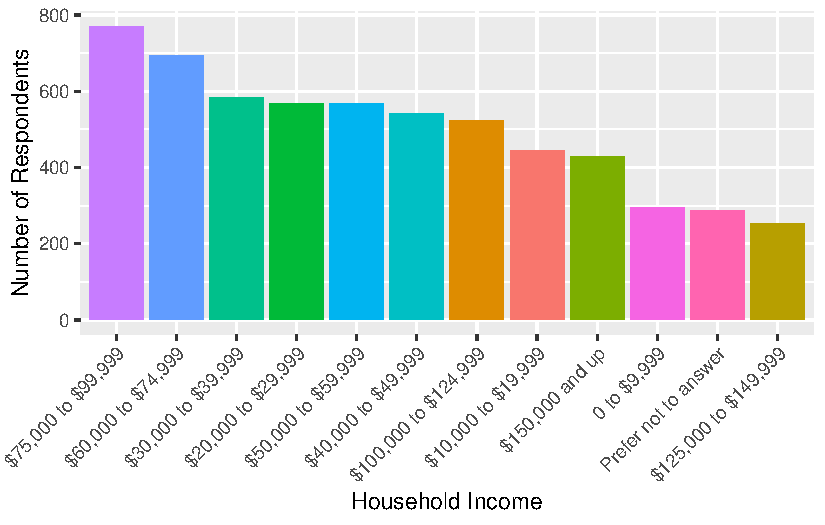
\includegraphics{paper_files/figure-pdf/fig-figure1-1.pdf}

}

\caption{\label{fig-figure1}Distribution of Income from Responses in a
facebook ad}

\end{figure}%

\subsection{Ethnicity Data}\label{sec-race_data}

The second question of the data that we have included in our analysis is
the ethnicity of the respondents. This again is a categorical variable,
that the individual self identifies their own ethnicity. The response
options included Asian or Pacific Islander, White / Caucasian, Hispanic,
Black or African American and other. (\textbf{race\_dist?}) shows the
percentage of respondents in each with the overwhelming majority of
responses being Caucasian at nearly 70\%. This is actually less than the
most recent estimates by the United States government which estimate
over 75\% of the population is Caucasian (cite us gov). The data also
has an over representation of Asian and Native Americans. This results
in an under representation of Hispanic and African American populations.

https://www.census.gov/quickfacts/fact/table/US/PST045222

\begin{longtable}[]{@{}lr@{}}

\caption{\label{tbl-race\_dist}Percentage of each Ethnicity from
Responses in a facebook ad}

\tabularnewline

\toprule\noalign{}
Ethnicity & Percentage of Responses \\
\midrule\noalign{}
\endhead
\bottomrule\noalign{}
\endlastfoot
American Indian or Alaskan Native & 0.7554138 \\
Asian or Pacific Islander & 13.5806614 \\
Black or African American & 6.0936713 \\
Hispanic & 8.0577472 \\
Other (please specify) & 2.5851939 \\
White / Caucasian & 68.9273124 \\

\end{longtable}

\subsection{Politics Data}\label{sec-pol_data}

The third variable in the data that is included in our analysis is a
variable of respondents self identifying how closely they follow
politics. This is another categorical variable measured as Not at all
closely, Somewhat closely, Rather closely and Very closely. This
variable faces many problems as this categorical scale is not consistent
across respondents. To be specific we mean someone who identifies as
someone who does follows Not at all closely can be following politics
more than someone who identifies as Somewhat closely. This is a
measurement issue within to the questions asked in the survey and all
self identifying variables in general. (\textbf{figure2?}) shows the
quantity of respondents in each group. The most common response is that
they follow somewhat closely and the other responses are relatively
even.

\begin{figure}

\centering{

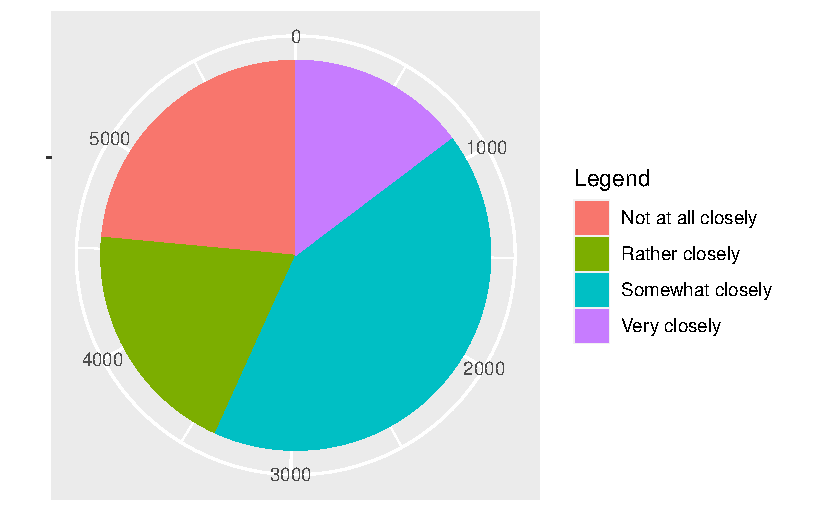
\includegraphics{paper_files/figure-pdf/fig-figure2-1.pdf}

}

\caption{\label{fig-figure2}How Closely People Follow Politics from
Responses in a facebook ad}

\end{figure}%

\subsection{Missing Data}\label{sec-Missing_data}

\begin{Shaded}
\begin{Highlighting}[]
\CommentTok{\# Parts of this code from R{-}charts}
\CommentTok{\#https://r{-}charts.com/part{-}whole/stacked{-}bar{-}chart{-}ggplot2/}
\CommentTok{\# Assisited by Chat GPT3.5 {-} view full chat in inputs/llms/usage.txt}
\FunctionTok{ggplot}\NormalTok{(cleaned\_data, }\FunctionTok{aes}\NormalTok{(}\AttributeTok{x =}\NormalTok{ follow\_trump, }\AttributeTok{fill =}\NormalTok{ race)) }\SpecialCharTok{+}
  \FunctionTok{geom\_bar}\NormalTok{(}\AttributeTok{position =} \StringTok{\textquotesingle{}stack\textquotesingle{}}\NormalTok{, }\AttributeTok{color =} \StringTok{\textquotesingle{}black\textquotesingle{}}\NormalTok{, }\AttributeTok{stat =} \StringTok{\textquotesingle{}count\textquotesingle{}}\NormalTok{) }\SpecialCharTok{+}
  \FunctionTok{labs}\NormalTok{(}\AttributeTok{title =} \StringTok{"Number of People Following Trump by Race"}\NormalTok{,}
       \AttributeTok{x =} \StringTok{"Follows Trump"}\NormalTok{,}
       \AttributeTok{y =} \StringTok{"Count"}\NormalTok{) }\SpecialCharTok{+}
  \FunctionTok{scale\_fill\_manual}\NormalTok{(}\AttributeTok{values =} \FunctionTok{c}\NormalTok{(}\StringTok{\textquotesingle{}White / Caucasian\textquotesingle{}} \OtherTok{=} \StringTok{\textquotesingle{}lightblue\textquotesingle{}}\NormalTok{, }\StringTok{\textquotesingle{}Black or African American\textquotesingle{}} \OtherTok{=} \StringTok{\textquotesingle{}lightcoral\textquotesingle{}}\NormalTok{, }\StringTok{\textquotesingle{}Asian or Pacific Islander\textquotesingle{}} \OtherTok{=} \StringTok{\textquotesingle{}lightgreen\textquotesingle{}}\NormalTok{, }\StringTok{\textquotesingle{}Hispanic\textquotesingle{}} \OtherTok{=} \StringTok{\textquotesingle{}plum\textquotesingle{}}\NormalTok{,}
                               \StringTok{\textquotesingle{}Other  (please specify)\textquotesingle{}} \OtherTok{=} \StringTok{\textquotesingle{}lightgoldenrodyellow\textquotesingle{}}\NormalTok{)) }\SpecialCharTok{+}
  \FunctionTok{theme\_minimal}\NormalTok{()}
\end{Highlighting}
\end{Shaded}

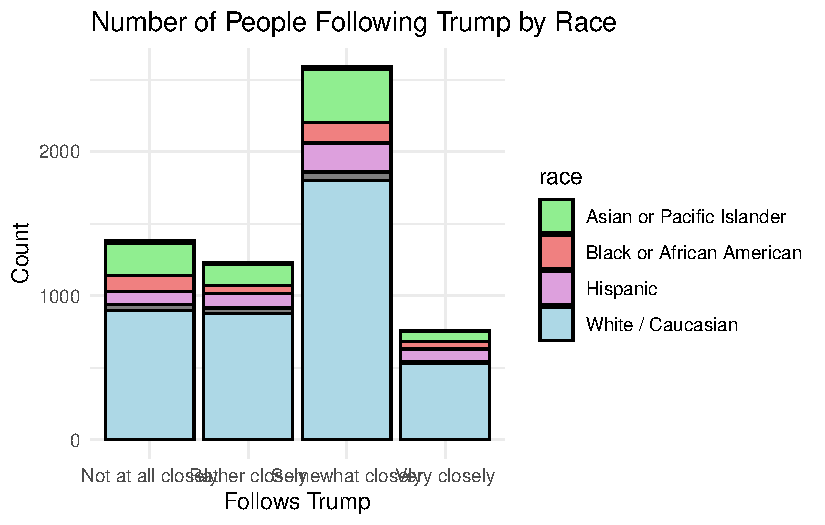
\includegraphics{paper_files/figure-pdf/unnamed-chunk-5-1.pdf}

\begin{figure}

\centering{

\captionsetup{labelsep=none}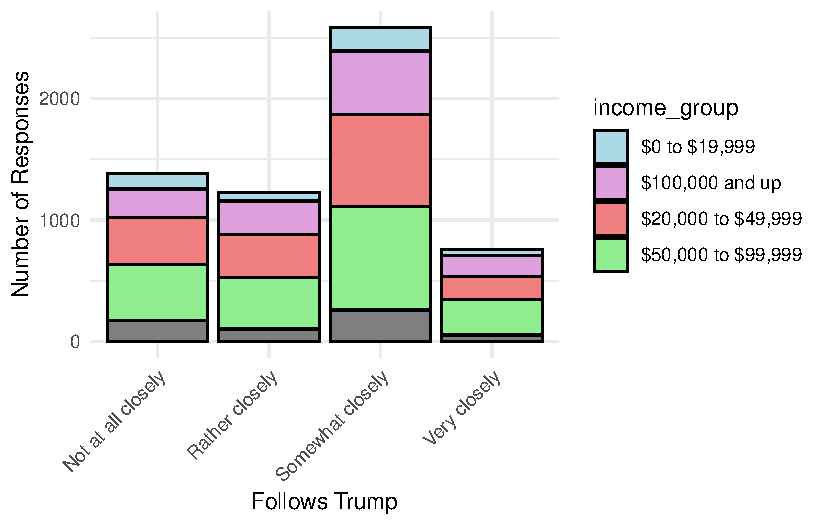
\includegraphics{paper_files/figure-pdf/fig-figure3-1.pdf}

}

\caption{\label{fig-figure3}}

\end{figure}%

\section{Model}\label{model}

simple regression of income and politics data controlling for race

\section{Discussion}\label{discussion}

like to incluse variables like state etc data set too small/ incomplete
for that \#\# First discussion point \{\#sec-first-point\}

If my paper were 10 pages, then should be be at least 2.5 pages. The
discussion is a chance to show off what you know and what you learnt
from all this.

\subsection{Second discussion point}\label{second-discussion-point}

\subsection{Third discussion point}\label{third-discussion-point}

\subsection{Weaknesses and next steps}\label{weaknesses-and-next-steps}

Weaknesses and next steps should also be included.

\newpage

\appendix

\section*{Appendix}\label{appendix}
\addcontentsline{toc}{section}{Appendix}

\section{Additional data details}\label{additional-data-details}

\section{Model details}\label{sec-model-details}

\newpage

\section*{References}\label{references}
\addcontentsline{toc}{section}{References}

\phantomsection\label{refs}
\begin{CSLReferences}{1}{0}
\bibitem[\citeproctext]{ref-citeLahman}
Friendly, Michael, Chris Dalzell, Martin Monkman, and Dennis Murphy.
2020. \emph{Lahman: Sean {``Lahman''} Baseball Database}.
\url{https://CRAN.R-project.org/package=Lahman}.

\bibitem[\citeproctext]{ref-gebru2021datasheets}
Gebru, Timnit, Jamie Morgenstern, Briana Vecchione, Jennifer Wortman
Vaughan, Hanna Wallach, Hal Daumé Iii, and Kate Crawford. 2021.
{``Datasheets for Datasets.''} \emph{Communications of the ACM} 64 (12):
86--92.

\bibitem[\citeproctext]{ref-rstanarm}
Goodrich, Ben, Jonah Gabry, Imad Ali, and Sam Brilleman. 2022.
{``Rstanarm: {Bayesian} Applied Regression Modeling via {Stan}.''}
\url{https://mc-stan.org/rstanarm/}.

\bibitem[\citeproctext]{ref-palmerpenguins}
Horst, Allison Marie, Alison Presmanes Hill, and Kristen B Gorman. 2020.
\emph{Palmerpenguins: Palmer Archipelago (Antarctica) Penguin Data}.
\url{https://doi.org/10.5281/zenodo.3960218}.

\bibitem[\citeproctext]{ref-citeR}
R Core Team. 2022. \emph{R: A Language and Environment for Statistical
Computing}. Vienna, Austria: R Foundation for Statistical Computing.
\url{https://www.R-project.org/}.

\bibitem[\citeproctext]{ref-thereferencecanbewhatever}
Wickham, Hadley, Mara Averick, Jennifer Bryan, Winston Chang, Lucy
D'Agostino McGowan, Romain François, Garrett Grolemund, et al. 2019.
{``Welcome to the {tidyverse}.''} \emph{Journal of Open Source Software}
4 (43): 1686. \url{https://doi.org/10.21105/joss.01686}.

\end{CSLReferences}



\end{document}
